% vim: spelllang=en_gb

\documentclass[12pt,a4paper,draft]{scrartcl}
\usepackage{ifdraft}

% --------------------
% Set Language Options
% --------------------

\usepackage[nswissgerman,french,main=english]{babel}
\usepackage[autostyle,english=american,german=swiss]{csquotes}
\MakeOuterQuote{"}

\usepackage[shortcuts]{extdash}

% --------------
% Font & Symbols
% --------------

\usepackage{amssymb,mathtools}
\usepackage[warnings-off={mathtools-colon,mathtools-overbracket}]{unicode-math}
\usepackage[oldstyle,proportional]{libertinus-otf}

% ---------------
% Set Page Layout
% ---------------

% Get length of 65 characters
%\setlxvchars

\usepackage[driver=auto]{geometry}
% A5: 148mm × 210mm
% A4: 210mm × 297mm
\geometry{
  width=140mm,
  height=217mm,
  marginparsep=3mm,
  marginparwidth=30mm,
}
\ifdraft{\geometry{
  inner=10mm,
  marginparwidth=50mm
}}{}


% ---------------------
% Load Various Packages
% ---------------------

% Various Math Environments
\usepackage{amsthm,thmtools}
\usepackage{physics} % various shortcuts

% Bibliography
\usepackage{biblatex}
\addbibresource{bibliography.bib}

% For general figures
\usepackage[final]{graphicx}
\graphicspath{{/img}}
\usepackage{subcaption}
\usepackage{tikz}
\usetikzlibrary{babel,cd,shapes,3d}
\tikzcdset{arrow style=math font}
\tikzset{cross/.style={
    cross out, draw, solid, thin, 
    minimum size=2*(#1-\pgflinewidth), 
    inner sep=0pt, outer sep=0pt
  },
  cross/.default={3},
  conic/.pic={
    \begin{scope}[canvas is xz plane at y=0]
      \draw (0,0) circle [radius=0.5];
    \end{scope}
    \begin{scope}[canvas is xz plane at y=1]
      \draw (0,0) circle [radius=0.8];
    \end{scope}
    \begin{scope}[canvas is xz plane at y=-1]
      \draw (-20:.8) arc [start angle=-20,end angle=160,radius=.8];
      \draw[dotted] (160:.8) arc [start angle=160,end angle=340,radius=.8];
    \end{scope}
    \begin{scope}[rotate around y=20]
      \draw (.8,1) .. controls +(0,0) and +(0,.3) .. (0.5,0) .. controls +(0,-0.3) and +(0,0) .. (.8,-1);
      \draw (-.8,1) .. controls +(0,0) and +(0,.3) .. (-0.5,0) .. controls +(0,-0.3) and +(0,0) .. (-.8,-1);
    \end{scope}
  },
  degenerate conic/.pic={
    \begin{scope}[canvas is xz plane at y=1]
      \draw (0,0) circle [radius=.8];
    \end{scope}
    \begin{scope}[canvas is xz plane at y=-1]
      \draw (-20:.8) arc [start angle=-20,end angle=160,radius=.8];
      \draw[dotted] (160:.8) arc [start angle=160,end angle=340,radius=.8];
    \end{scope}
    \begin{scope}[rotate around y=20]
      \draw (-.8,-1) -- (.8,1);
      \draw (-.8,1) -- (.8,-1);
    \end{scope}
  },
  reduced conic/.pic={
    \begin{scope}[canvas is xz plane at y=1]
      \draw[very thin, opacity=0.5] (0,0) circle [radius=.8];
      \draw (-32:.8) arc [start angle=-32,end angle=32,radius=.8];
    \end{scope}
    \begin{scope}[canvas is xz plane at y=-1]
      \draw[very thin, opacity=0.5] (0,0) circle [radius=.8];
      \draw (-32:.8) arc [start angle=-32,end angle=32,radius=.8];
    \end{scope}
    \begin{scope}[canvas is xz plane at y=0]
      \draw[very thin, opacity=0.5] (0,0) circle [radius=.5];
      \draw (-32:.5) arc [start angle=-32,end angle=32,radius=.5];
    \end{scope}
    \foreach \φ in {32,-32} {
      \begin{scope}[rotate around y=\φ]
        \draw (.8,1) .. controls +(0,0) and +(0,.3) .. (0.5,0) .. controls +(0,-0.3) and +(0,0) .. (.8,-1);
      \end{scope}
    }
    \begin{scope}[rotate around y=20]
      \draw[very thin, opacity=0.5] (-.8,1) .. controls +(0,0) and +(0,.3) .. (-0.5,0) .. controls +(0,-0.3) and +(0,0) .. (-.8,-1);
    \end{scope}
  }
}

% For lists
\usepackage[shortlabels]{enumitem}

% For better Tables
\usepackage{tabularray}

% For more fine grained typesetting in final mode.
% Else set the tolerance for overfull warnings higher.
\ifdraft{\hfuzz=1.5pt}{\usepackage{microtype}}

% Links and stuff
\usepackage[final]{hyperref}
\usepackage[noabbrev,capitalize]{cleveref}

% For Todonotes
\usepackage[obeyDraft]{luatodonotes}

% --------------------------------------------
% Define Theorem Environments & Math Operators
% --------------------------------------------

\declaretheorem[numberwithin=section]{theorem}
\declaretheorem[sibling=theorem]{lemma, proposition, corollary}
\declaretheorem[sibling=theorem,style=definition]{definition, example}
\declaretheorem[sibling=theorem,style=remark]{remark}

\DeclareMathOperator{\id}{id}
\DeclareMathOperator{\im}{im}
\DeclareMathOperator{\Aut}{Aut}
\DeclareMathOperator{\Diff}{Diff}
\DeclareMathOperator{\GL}{GL}
\DeclareMathOperator{\HF}{HF}
\DeclareMathOperator{\HM}{HM}
\DeclareMathOperator{\Hom}{Hom}
\DeclareMathOperator{\Ext}{Ext}
\DeclareMathOperator{\Tor}{Tor}
\DeclareMathOperator{\Flux}{Flux}

\begin{document}
\title{Semi-Local Lagrangian Tori in Dimension Four}
\author{JoJoJo}

\maketitle

\section{Introduction}

\begin{definition}
  Let $k ∈ ℕ$ such that $0<k≤d$ and $a ∈ (0,∞)$. Through nodal slides we can arrange the ATF on $B_{dpq}$ such that the line $x₂=a$ intersects the branch cut line between the $(k-1)$-th and $k$-th degenerated fibre. $T_k(a)$ is defined to be the fibre over the intersection point of these two lines.
\end{definition}

\begin{restatable}{theorem}{thmbdpqexotic}
    \label{thm:bdpqexotic}
  Let $U ⊂ H¹(T_k(a);ℝ) ∖ \{\text{branch cut line}\}$.
  Up to a change of basis, the restriction of the displacement energy germ to $U$ is given by
  \[ \eval{\symcal{E}_{T_k(a)}}_U (x,y) = a+\min\{x,x(1-kpq)+ykp²\} \]
\end{restatable}

\section{Fun facts über ATFS by Joé}

\begin{lemma}
  \label{thm:nodal_slide}
  Nodal slides geben symplektomorphismus supported auf umgebung von geslideten nodes.
\end{lemma}


\section{Construction of the Local Model}
\label{sec:construction}

Let $d,p,q$ integers such that $d≥1$ and $p,q$ coprime\footnote{We consider the pair $(1,0)$ as coprime.} with $p>q≥0$, and $0<a_1<…<a_d ∈ ℝ$.
Let $P ∈ ℂ[z]$ be the polynomial $P(z) = \prod_{i=1}^d (z^p-a_i)$.
Define the complex manifold $M_P$ by
\begin{equation}
  \label{eqn:MP}
M_P = \qty{(z_1,z_2,z_3) ∈ ℂ³ \mid z₁z₂ + P(z₃)=0 } \; ,
\end{equation}
with the natural symplectic and complex structure inherited from $ℂ³$.

We define the pair of Poisson commuting Hamiltonian functions $\symbf{H} \colon ℂ^3 → ℝ^2$
\begin{equation}
  \label{eqn:non-toric-system}
  \symbf{H}(z_1,z_2,z_3) = \qty(\abs{z_3}^2, \frac{1}{2}\qty(\abs{z_1}^2-\abs{z_2}^2)) \; .
\end{equation}

Let $G_p$ be the group of $p$-th roots of unity acting on $M_P$ by
\[g \cdot (z₁,z₂,z₃) = \qty(gz₁,g^{-1}z₂,g^q z₃), \quad g ∈ G_p \; .\]
This is a free  action, so the quotient $B_{P,q} = M_P/G_p$ is a smooth complex and symplectic manifold.
$\symbf{H}$ is invariant under the action, so $\symbf{H}$ descends to a well defined pair of Poisson commuting Hamiltonians on $B_{P,q}$, giving us the fibration (by abuse of notation also called $\symbf{H}$) $\symbf{H} \colon B_{P,q} → B = \im(\symbf{H}) ⊂ ℝ^2$.
Up to symplectomorphism, the space $M_P$ (and thus also $B_{P,q}$) is independent of the choice of $P$. This follows either for standard Moser-type arguments, or from \cref{thm:nodal_slide} using the almost toric fibration on $B_{P,q}$ which will be constructed in \cref{sec:Bdpqatfs}. So unless necessary we will denote $B_{P,q}$ by $B_{dpq}$.

\begin{remark}
  Was ist der raum $B_dpq$? $ℚ$-gorenstein smoothing of cyclic quotient T-singularity $\frac{1}{dp^2}(1,dpq-1)$… Referenzen?
\end{remark}

\begin{figure}
  \centering
  \begin{tikzpicture}[scale=0.7]
    \begin{scope}[shift={(-4.25cm,0)}]
      \begin{scope}[canvas is xz plane at y=0]
        \fill[green,opacity=0.2] (-4,-4) rectangle (4,4);
        \clip (-4,-4) rectangle (4,4);
        \foreach \φ in {0,72,144,216,288} {
          \draw[opacity=0.4] (0,0) -- (\φ:6);
          \foreach \x in {1,2,3} \draw (\φ:\x) circle [radius=1pt];
        }
        \draw[very thin] (0,0) circle [radius=3];
      \end{scope}
      \begin{scope}[canvas is xz plane at y=2]
        \foreach \φ in {0,72,144,216,288} {
          \draw[purple] (\φ:3) .. controls (\φ+36:3+0.3) .. (\φ+72:3) .. controls (\φ+36:3-0.3) .. (\φ:3);
        }
      \end{scope}
      \foreach \φ in {0,72,144,216,288} {
        \begin{scope}[rotate around y=\φ]
          \draw (3,2,0) pic[scale=0.5, transform shape, rotate around y=-\φ]{degenerate conic};
          \draw[very thin] (3,1.3,0) -- (3,0,0);
        \end{scope}
      }
      \node at (-1,-2.25) {(a) A degenerate "pinched torus" fibre of $\symbf{H} \colon M_P → B$};
    \end{scope}
    \begin{scope}[shift={(4.25cm,0)}]
          \begin{scope}[canvas is xz plane at y=0]
          \fill[green,opacity=0.2] (-4,-4) rectangle (4,4);
          \clip (-4,-4) rectangle (4,4);
          \foreach \φ in {0,72,144,216,288} {
            \draw[opacity=0.4] (0,0) -- (\φ:6);
            \foreach \x in {1,2,3} \draw (\φ:\x) circle [radius=1pt];
          }
          \draw[very thin] (0,0) circle [radius=3.5];
        \end{scope}
        \begin{scope}[canvas is xz plane at y=2]
          \draw[purple] (0,0) circle [radius=3.5+0.2] circle [radius=3.5-0.2];
        \end{scope}
        \foreach \φ in {0,72,144,216,288} {
          \begin{scope}[rotate around y=\φ]
            \draw (3.5,2,0) pic[scale=0.4, transform shape, rotate around y=-\φ]{conic};
            \draw[very thin] (3.5,1.3,0) -- (3.5,0,0);
          \end{scope}
        }
        \node at (-1,-2.25) {(b) A regular fibre of $\symbf{H} \colon M_P → B$.};
    \end{scope}
    \begin{scope}[shift={(0,-5.5cm)}]
      \begin{scope}[canvas is xz plane at y=0]
        \fill[green,opacity=0.2] (-4,-4) rectangle (4,4);
        \clip (-4,-4) rectangle (4,4);
        \foreach \φ in {0,72,144,216,288} {
          \draw[opacity=0.4] (0,0) -- (\φ:6);
          \foreach \x in {1,2,3} \draw (\φ:\x) circle [radius=1pt];
        }
      \end{scope}
      \draw (0,2,0) pic[scale=0.3] {conic};
      \foreach \φ in {0,72,144,216,288} {
        \begin{scope}[rotate around y=\φ]
          \foreach \x in {1,2,3}
          \draw[very thin, opacity = 0.5] (\x,0,0) -- (\x,2,0);
        \end{scope}
      }
      \begin{scope}[canvas is xz plane at y=2]
        \foreach \φ in {0,72,144,216,288} {
          \begin{scope}[rotate=\φ]
            \foreach \d in {-0.2,0.2} {
              \draw[red] (0,\d) .. controls +(0.5,0) and +(0,0) .. (1,0);
              \draw[purple] (1,0) .. controls +(.5,1.5*\d) .. (2,0);
              \draw[blue] (2,0) .. controls +(.5,1.5*\d) .. (3,0);
%              \draw (0,\d) -- (3,\d);
            }
          \end{scope}
        }
      \end{scope}
      \node at (-1,-2.25) {(c) The Lagrangians $\hat{S}_k ⊂ M_P$};
    \end{scope}
\end{tikzpicture}
  \caption{The projection $M_P ∋ z ↦ z_3$ for $p=5$, $d=3$.}
  \label{fig:conic_fibration}
\end{figure}

\subsection{Almost toric fibrations}
\label{sec:Bdpqatfs}

Let us further inspect the fibration $\symbf{H} \colon B_{dpq} → B$. To this end, we look at the projection $π_3 \colon M_P → ℂ$ onto the $z_3$ coordinate, see \cref{fig:conic_fibration} (a) and (b).
The fibre over a point $z_3$ is given by $z_1 z_2 - P(z_3) = 0$, so if $P(z_3) ≠ 0$ this is a cylinder in $ℂ^2 × \{z_3\}$ (as seen in \cref{fig:conic_fibration} (b)), and if $P(z_3) = 0$, this is $(ℂ × \{0\} ∪ \{0\} × ℂ) × \{z_3\}$, i.e.\ the transverse intersection of the $z_1$ and $z_2$ planes (as seen in \cref{fig:conic_fibration} (a)).
Fix $b = (b_1,b_2) ∈ B$. For $b_1 ≠ 0$, the set $\symbf{H}_1^{-1}(b_1)$ gives us a circle in the $z_3$ plane, and the intersection with $\symbf{H}_2^{-1}(b_2)$ fixes a "height" in the cylinders.
Thus if $b$ is a regular value, $\symbf{H}^{-1}(b)$ is a torus, as in \cref{fig:conic_fibration} (b).
There are two kinds of degenerate values: The elliptic-regular with $b_1=0$, where $\symbf{H}^{-1}(0,b_2)$ is a circle, and focus-focus with $b = ({a_k}^{2/p},0)$ where $\symbf{H}^{-1}(b)$ is a torus with $p$ pinched circles, as in \cref{fig:conic_fibration} (a). \todo{Warum ist $\symbf{H}$ eine almost toric fibration?}

Note that the intersection $\hat{S}_k = ⋃_{ρ ∈ ρ_p} π_3^{-1}([ρ a_k^{2/p},ρ a_{k+1}^{2/p}]) ∩ \symbf{H}_2^{-1}(0)$ forms a collection of $p$ Lagrangian
\footnote{They are contained in the fixed point set of an (anti-)symplectic involution, see \cite[Remark 7.10]{evans2021atfs} for details.}
disks for $k=0$ and spheres for $0<k<d$, with the disks intersecting on their boundary $\{z_3=0,\symbf{H}_2=0\}$, see \cref{fig:conic_fibration} (c).

\begin{figure}
  \centering
  \begin{tikzpicture}[scale=1.5]
    \begin{scope}[canvas is xz plane at y=0]
      \fill[green,opacity=0.2] (0,0) -- (32:4) arc[start angle=32,end angle=-32,radius=4] -- (0,0);
      \draw[opacity=0.4] (0,0) -- (4,0);
      \draw[very thin] (32:3) arc[start angle=32,end angle=-32,radius=3];
      \draw (0,0) node[cross] {} \foreach \x in {1,2,3} {(\x,0) circle[radius=1pt]};
    \end{scope}
    \begin{scope}[canvas is xz plane at y=2]
      \foreach \d in {0.2,-0.2}
      \draw[purple] (-32:3+\d) .. controls (-16:3+\d) .. (0:3) .. controls (16:3+\d) .. (32:3+\d);
    \end{scope}
    \draw (0,2,0) pic[scale=0.4,transform shape] {reduced conic};
    \draw (3,2,0) pic[scale=0.4,transform shape] {degenerate conic};
    \draw[very thin] (0,0,0) -- (0,1.3,0);
    \draw[very thin] (3,0,0) -- (3,1.3,0);
  \end{tikzpicture}
  \caption{A fundamental domain of the quotient $B_dpq$ of $M_P$ by $G_p$}
  \label{fig:conic_fibration_fundamental_domain}
\end{figure}

Under the reduction $M_P/G_p$, a conic fibre $π_3^{-1}(z_3)$ will be identified with the fibre $π_3^{-1}(g^q z_3)$ under the map $(z_1,z_2) ↦ (gz_1,g^{-1}z_2)$.
Consider the fundamental domain in \cref{fig:conic_fibration_fundamental_domain} of this action obtained by restricting $z_3 = re^{iθ} ∈ M_P$ to $θ \in [-\frac{π}{p},\frac{π}{p}]$, and $π_3^{-1}(0) ∋ (z_1,z_2)$ to $\frac{1}{2}\arg\qty(\frac{z_1}{z_2}) ∈ [-\frac{π}{p},\frac{π}{p}]$.
Let $g = e^{2πi/p}$ a generator of $G_p$.
The cylinders $π_3^{-1}(z_3)$ with $θ=-\frac{π}{p}$ and $r>0$ are identified with the cylinders $π_3^{-1}(g z_3)$ by the map $(z_1,z_2) ↦ (g^{q'} z_1,g^{-q'} z_2)$, where $q'$ is chosen s.t.\ $qq' = 1 \mod p$.

The image $S_k = \hat{S}_k / G_p$ is a Lagrangian sphere for $0<k<d$, and a Lagrangian disk with its boundary identified by the map $z ↦ g^{q'} z$. $S_0$ is called a Lagrangian pinwheel and denoted $L_{p,q}$. On the fibre $π_3(0)$, there are $p$ flanges meeting, such that one turn around the circle shifts the identification of the flanges by $q'$ places. See \cref{fig:pinwheel}.

\begin{figure}
  \centering
  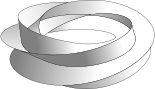
\includegraphics[width=0.7\textwidth]{img/pinwheel2.pdf}
  \caption{The "core" of the Lagrangian pinwheel $S_0 = L_{q,p}$. The pinwheel is obtained by glueing the boundary to a point. (Here $p=5,q=2$)}
  \label{fig:pinwheel}
\end{figure}

\begin{lemma}
  Let $ℓ = [a_1^{2/p},∞] × \{0\}$. Then there is a smooth map $τ: B ∖ ℓ → Δ = \{(u,v) ∈ ℝ² \mid u ≥ 0 \}$, such that $μ = τ ∘ \symbf{H} \colon B_{dpq} → Δ$:
\end{lemma}

To calculate the image of $B_{dpq}$ under action-angle coordinates, we can remove the segment $ℓ = [a_1^{2/p},∞] × \{0\}$ from $\im(\symbf{H})$ to obtain a simply connected domain of regular or elliptic-regular values of $\symbf{H}$.
Now applying the flux map\todo{Das ganze nach die Versal deformation section?} gives us a smooth map $τ \colon \im(\symbf{H}) ∖ ℓ → Δ ⊂ ℝ²$, where we define $Δ ⊂ ℝ²$ to be the image of this map, and thus giving us action-angle coordinates $μ \colon B_{dpq} ∖ \symbf{H}^{-1}(ℓ) → Δ$.
Since $\symbf{H}_2$ already generates a $S¹$ action, we may choose $τ$ to be of the form $τ(b_1,b_2) = (τ_1(b_1,b_2), b_2)$.\footnote{As when constructing action-angle coordinates in the proof of the Arnold-Liouville Theorem.}
In particular the segment $[0,a_1^{2/p}] × \{0\}$ is mapped to $[0,τ_1(a_1^{2/p},0)] × \{0\}$, even more particular $S_0$ is a Lagrangian over this segment, making it a so-called visible Lagrangian as described in \cite[Chapter 5]{evans2021atfs}.
We also know that the line $\{0\} × ℝ ⊂ \im(\symbf{H})$, consisting of elliptic-regular singularities, is sent to a straight line in some rational direction $(n,m)$.
As we have the visible Lagrangian pinwheel $S_0 = L_{p,q}$ intersecting it, by \cite[Section 5.3]{evans2021atfs}, we must have $(n,m) = (q',p)$.
After the affine linear transformation $\mqty(p & -q'\\q & p')$, with $p' = \frac{1-qq'}{p}$, the image of $τ$ is the right half plane, with the nodes sitting on a ray in direction $(p,q)$ as in \cref{fig:Bdpq_moment_image}.

Note that $μ$ can be continuously extended over all of $B_{dpq}$, even for points in $\symbf{H}^{-1}(ℓ)$. \todo{MEEHHHR details.}


\begin{figure}
  \centering
  \begin{tikzpicture}[scale=.7]
    \begin{scope}[shift={(-5cm,0)}]
        \fill[blue,opacity=0.2] (0,4) rectangle (8,-1);

        \draw (2,1.5) node[cross] {} (4,1.5) node[cross] {} (6,1.5) node[cross] {};
        \draw[thick] (0,4) -- (0,-1);
    \end{scope}
    \begin{scope}[shift={(5cm,0)}]
        \fill[opacity=0.1] (0,4) rectangle (8,-1);

        \draw[thick,dotted,->] (2,1) node[cross] {} -- (4,2) node[cross] {} -- (6,3) node[cross] {} -- (8,4) node[anchor=west] {$(p,q)$};
        \draw[thick] (0,4) -- (0,-1);
    \end{scope}
  \end{tikzpicture}
  \caption{Moment image of $B_{dpq}$ under $μ$}
  \todo{Kommentieren, was $\symbf{H}$ is und was $\mu$ ist.}
  \label{fig:Bdpq_moment_image}
\end{figure}


\subsection{Homology of \texorpdfstring{$B_{dpq}$}{Bdpq}}
\label{sec:homology}

In order to calculate the lower bound for the displacement energy of a Lagrangian torus fibre $T(b) = μ^{-1}(\qty{b})$ for $b ∈ \im(\symbf{H})$, we will want to have calculated a basis of the homology $H_2\qty(B_{dpq},T(b))$.

$B_{dpq}$ deformation retracts to the preimage under $\symbf{H}$ of the branch cut line segment $ℓ$ shown in red in \cref{fig:branch_cut_retraction}: We first vertically retract the space onto the preimage under $\symbf{H}$ of the ray $[0,∞) × \{0\}$ (for example by flowing along the Morse-Bot function $|\symbf{H}_2|^2$).
Thus we may assume that $b$ lies somewhere on that line. For illustration purposes only we assume that $b_1> |a_d|^{1/p}$, that is $b$ lies to the right of any nodes in $B$. and then compressing the part of the ray that is to the right of all the critical points.
\todo{Das ist etwas dumm formuliert, lohnt es sich das besser zu formulieren?}

The preimage $\symbf{H}^{-1}(ℓ)$ can be understood as follows: If there were no critical points on the line, this would be a solid torus $\hat{T} = S¹×D²$ with $∂ \hat{T} = T(b)$.
We pick $(1,0),(0,1) ∈ H₁(∂ \hat{T})$ to be the classes generated by the orbits of Hamiltonian flows of $μ_1$ and $μ_2$ respectively.
For each critical fibre $k ∈ \qty{1,…,d}$ we collapse a loop along the homology class $(-q,p)$, as in \cref{fig:collapse_cycles}.
Up to homotopy this is the same as attaching a disk $D_k$ along $(-q,p)$.
Again up to homotopy we can also require that the $d$ discs $D_1,…,D_d$ are attached along $∂ \hat{T}$.
Let us call the resulting space $S$.

\begin{figure}
  \centering
  \begin{subfigure}{0.45\textwidth}
    \centering
    \begin{tikzpicture}[scale=1.8]
      \fill[blue,opacity=0.2] (0,1) rectangle (3,-1);
      \draw[thick] (0,1) -- (0,-1);
      \draw[line width=0.08cm,red,opacity=0.4,text opacity=1] (0,0) -- node[pos=0.6, anchor=north] {$ℓ$} (2.5,0);
    \fill (2.5,0)  circle[radius=1pt] node[anchor=south] {$T(b)$};
      \draw (1,0) node[cross] {} (2,0) node[cross] {};
    \end{tikzpicture}
    \caption{Retraction to branch cut line}
    \label{fig:branch_cut_retraction}
  \end{subfigure}%
  \begin{subfigure}{0.55\textwidth}
    \includegraphics[width=\textwidth]{img/homology_collapse.pdf}
    \caption{The two cycles marked in red and purple (here $p=2, q=1$) are collapsed to a point.}
    \label{fig:collapse_cycles}
  \end{subfigure}
  \caption{Calculation of the homology of $B_{dpq}$}
\end{figure}

Let us look at the long exact sequence of homology for the pair $\qty(B_{dpq},T(x_1,x_2))$. This pair is homotopy equivalent to $(S,∂ \hat{T})$.

\[
\begin{tikzcd}
  H_2(∂ \hat{T}) \ar[r,"0"] &
  H_2(S) \ar[r,hook]\ar[d,"≅"] &
  H_2(S,∂ \hat{T}) \ar[r]\ar[d,"≅"] &
  H_1(∂ \hat{T}) \ar[r]\ar[d,"≅"] &
  H_1(S) \ar[d,"≅"]
  \\
  &
  ℤ^{d-1} &
  ℤ^{d+1} &
  ℤ² &
  ℤ_p
\end{tikzcd}
\]

The first horizontal map is zero since $∂ \hat{T}$ retracts to a circle in $S$.
The homology $H_2(S)$ can be seen as follows: By contracting the solid torus $\hat{T}$ in $S$ to a circle, we see that $S$ is homotopic to a circle with $d$ discs glued to its boundary by a degree $p$ map.
So $H_2(S)$ is generated by spheres $\qty{S_2,…,S_d}$, $S_k = D_{k-1}-D_{k}$.
$H_2(S,∂ \hat{T})$ is generated by the discs $D_0 = \text{pt}×D²,D₁,…,D_d$. In $B_{dpq}$, these discs can be seen, where the disc intersecting the toric boundary collapses the $(0,1)$ cycle in the toric fibre $T(x_1,x_2)$ and the discs intersecting the critical points collapse the $(-q,p)$ cycle (see \cref{fig:homology_generating_discs}).
The elements $S_2,\ldots,S_d \in H_2(B_{dpq})$ can be realized by embedded Lagragian spheres fibering over the segments between the nodes in the ATF -- these are so-called \emph{visible Lagrangians}, see \cite[Section 7.4]{evans2021atfs}.
The boundary map $∂ \colon H_2(S,∂ \hat{T}) → H_1(∂ \hat{T})$ is given by $\partial D_0 = (0,1),\, \partial D_i = (-q,p)$, meaning that the last horizontal map $H_1(∂ \hat{T}) → H_1(S)$ maps $(0,1)$ to the generator of $ℤ_p$.


\begin{figure}
  \centering
  \begin{tikzpicture}
    \fill[black!5] (0,4) rectangle (7,-1);

    \coordinate (xy) at (2.7,3.5);
    \node[anchor=south] at (xy) {$T(x_1,x_2)$};
    \fill (xy) circle[radius=.05];
    \draw (xy)
           .. controls +(0,0) and +(-.5,1) .. node[anchor=east, near end] {$D₁$} (2,1)
      (xy) .. controls +(0,0) and +(-.5,1) .. node[anchor=west, near end] {$D₂$} (4,2)
      (xy) .. controls +(0,0) and +(-.5,1) .. node[anchor=west, near end] {$D₃$} (6,3)
      (xy) .. controls +(0,0) and +(1,0) .. node[anchor=south, near end] {$D₀$} (0,2.5);

    \draw[ultra thick, blue, draw opacity=.3] (2,1) -- node[anchor=north] {$S₂$} (4,2);
    \draw[ultra thick, purple, draw opacity=.3] (4,2) -- node[anchor=north] {$S₃$} (6,3);

    \draw[thick,dotted] (2,1) node[cross] {} -- (4,2) node[cross] {} -- (6,3) node[cross] {} -- (7,3.5);

    \draw[thick] (0,4) -- (0,-1);
  \end{tikzpicture}

  \caption{The disks $D₀, …, D_d$ generating the homology $H₂\qty(B_{dpq}, T(x_1,x_2))$}
  \label{fig:homology_generating_discs}
\end{figure}

\section{Lower Bound on Displacement Energy: Minimal J-holomorphic Curves}
\label{sec:lower_bound}

We want to use the following theorem by Chekanov \cite{chekanov1998} for a lower bound of the displacement energy

\begin{theorem}
  \label{thm:chekanov}
  Let $(X,ω,J)$ be a geometrically bounded\todo{def.} symplectic manifold with $ω$-tame almost complex structure $J$\todo{Was sind die bedingungen an $J$}. Let $L ⊂ X$ be a compact Lagrangian submanifold. Then the displacement energy satisfies
  \[e(L) ≥ \min\qty{σ_D(X,L,J),σ_S(X,J)}\]
\end{theorem}
\todo{Why is $B_{dpq}$ geometrically bounded?}

To use \cref{thm:chekanov}, we can choose a suitable almost complex structure on $B_{dpq}$.

We do so in the following way: In the the construction of $B_{dpq}$ in \cref{sec:construction}, we defined $B_{dpq}$ as the quotient of $M_P$ under the free action of $ρ_p$. As a algebraic hypersurface $M_P$ naturally inherits the complex structure of $ℂ³$, and we use $J$ to denote this structure on $M_P$ as well as on its quotient $B_{dpq}$.

\begin{definition}
  Let $(M,J)$ be a almost complex manifold.
  A (smooth) function $f\colon (M,J) → ℂ$ is weakly plurisubharmonic if
  \[-d d^ℂ f = -d(d f ∘ J) ≥ 0 \;.\]
\end{definition}

The first component of $\symbf{H}$ in \ref{eqn:non-toric-system}, is a weakly plurisubharmonic function on $ℂ³$, as $-d d^ℂ \symbf{H}₁ = 2 d{x_3} ∧ d{y_3} ≥ 0$. As $M_P$ is an algebraic hypersurface, this restricts to a plurisubharmonic function on $M_P$, and also descends to the quotient $B_{dpq}$ as a plurisubharmonic function.

In particular, any $J$-holomorphic curve $u\colon Σ → B_{dpq}$ satisfies the maximum principle with respect to $\symbf{H}₁$, i.e.\ if $\symbf{H}₁ ∘ u$ has a maximum, it must be on $∂Σ$, and if $\symbf{H}₁ ∘ u$ is non-zero then it must be constant.\footnote{The latter is obtained by applying the maximum principle to $\frac{1}{\symbf{H}₁ ∘ u}$.}

\subsection{Non-Embedded lower bound}

Let $b = (b₁,b₂) ∈ \im(\symbf{H})$ and set $T = \symbf{H}^{-1}(b)$. Let $u \colon (Σ,∂Σ) → (B_{dpq},T)$ be a $J$-holomorphic curve. We have $\symbf{H}₁ ∘ u ≤ b₁$ by the maximum principle, thus $u$ is entirely contained in the region $\symbf{H}^{-1}(\qty{\symbf{H}₁ ≤ b₁})$. If we have $b₁ ≤ \symbf{H}₁(aᵢ)$, for all $1≤i≤d$, where the $a_i$ are the zeros of $P$ as in \cref{sec:homology}, then this region is homotopic to a solid torus.

Since the homology of $(\symbf{H}^{-1}(\qty{\symbf{H}_1 ≤ b_1}), T)$ is isomorphic to $ℤ$ and generated by $D₀$ as in \cref{sec:homology}, and the area of a $J$-disc rel $T$ only depends on its homology class, we have that
\[σ_D(X,T,J) ≥ ∫_{D₀} ω  = μ₁(T)\]

Since $B_{dpq}$ contains no $J$-holomorphic spheres,\footnote{As seen in \cref{sec:homology} the homology of $B_{dpq}$ is generated by Lagrangian spheres, thus any closed $J$-holomorphic curve has symplectic area $0$ and must be constant.} we have proven the following:

\begin{lemma}
  \label{thm:lower_bound_tmp}
  If $b₁ < \symbf{H}₁(aᵢ)$ for all $1 ≤ i ≤ d$, then
  \[e(B_{dpq},T) ≥ σ_D(X,T,J) ≥ ∫_{D₀} ω  = μ₁(T) \; .\]
\end{lemma}

Actually, since we are free to choose another almost complex structure, we can improve this result: 
Using a nodal slide on the moment image $μ$ as in \cref{thm:nodal_slide} we may construct a symplectomorphism $B_{P_1,q} → B_{P_2,q}$ which is a fibre-wise outside a neighbourhood of the line $\symbf{H}^{P_k,q}_2=0$, where $P_k$ are two polynomials each with $d$ distinct roots of multiplicity $p$.
For a torus $\symbf{H}^{-1}(b)$ with $b_2 ≠ 0$ we may therefore always change to a different polynomial $P_2$ where $b_1 < \symbf{H}_1(a_i)$, and choose the pullback of the natural almost complex structure of $B_{P_2,q}$. So we obtain:

\begin{lemma}
  \label{thm:lower_bound}
  If $b_2 ≠ 0$ then $e(B_{dpq},T) ≥ σ_D(X,T,J) ≥ μ₁(T)$.
\end{lemma}

\subsection{Embedded lower bound}

Let $(M,ω,J)$ be a geometrically bounded connected symplectic manifold with $ω$-tame almost complex structure $J$, denote by $g$ the associated Riemannian metric, and let $u\colon Σ → M$ be a J-holomorphic curve.

Then monotonicity (e.g. \cite[Proposition 4.3.1 (ii)]{sikorav1994}) gives us the following statement:

\begin{lemma}[Monotonicity]
  \label{thm:monotonicity}
  There exists a $C>0$ s.t.\ for all $x ∈ \im(u)$ and $B = B_r(x)$ the open ball w.r.t.\ $g$. If $u(∂Σ) ⊂ M ∖ B$ then we have
  \[∫_u ω ≥ C r²\]
\end{lemma}

As a simple corollary we get:

\begin{corollary}
  \label{cor:small_buffer}
  Suppose $∂M = ∂M^+ ⊔ ∂M^-$, with $∂M^±$ non-empty, $∂Σ = ∂Σ^+ ⊔ ∂Σ^-$, with $∂Σ^±$ non-empty and $u\colon (Σ,∂Σ) → (M,∂M)$ J-holomorphic with $u(∂Σ^±) ⊂ ∂M^±$, then
  \[∫_u ω ≥ \frac{C d(∂M^+,∂M^-)^2}{4} \; .\]
\end{corollary}

\begin{proof}
  Pick a path $γ$ from $∂Σ^-$ to $∂Σ^+$. By the intermediate value theorem there is $t$ s.t.\ $d((u ∘ γ) (t),∂M^+) = d((u ∘ γ)(t), ∂M^-)$. Picking $x = (u ∘ γ)(t)$ and using the triangle inequality we have that $B = B_{d(∂M^+,∂M^-)/2}(x) ⊂ M ∖ ∂M $. Applying \cref{thm:monotonicity} to $B$ we get the desired result.
\end{proof}

\begin{definition}
A \textbf{milnor fibre} of $B_{dpq}$ is a open subset $U$ containing $\symbf{H}^{-1}(ℓ)$, where $ℓ = [0,\symbf{H}(a_d)] × \{0\}$. \end{definition}

\begin{remark}
  This definition is a bit unusual but equivalent to the usual one.
\end{remark}

\begin{proposition}
  \label{thm:lower_bound_embedded}
  Let $φ:B_{dpq} ⊃ U → (X,ω)$ an embedding of a milnor fibre of $B_{dpq}$ into a tame symplectic manifold.

  Then there exists an $ε>0$, such that there exists a neighbourhood $V$ of $[0,ε) × \{0\} ⊂ \im{\symbf{H}}$ such that for all $b ∈ V$ with $b_2 ≠ 0$ we have $e(φ(T(b)),X) ≥ μ_1(T(b))$.
\end{proposition}

\begin{proof}
  Choose a smaller open neighbourhood $\symbf{H}^{-1}(ℓ) ⊂ U' ⊂ U$ such that $d(∂U',∂U) = s > 0$ and $U' = \symbf{H}^{-1}(V')$ for some open subset $V' ⊂ \im(\symbf{H})$ (this is possible since $\symbf{H}$ is an open map).
  Let $J$ be the natural almost complex structure on $B_{dqp}$ as in \cref{thm:lower_bound_tmp}, and $\hat{J}$ an extension of $φ_* J$ to all of $X$.


  The moment map $μ$ is given by $μ =  τ ∘ \symbf{H}$ for some diffeomorphism $τ$ defined on the complement of the branch cut line. Set $δ = \min\qty{σ_S(X,\hat{J}), \frac{Cs²}{4}}$, and set $V = V' ∩ τ^{-1}(μ_1 < δ)$.

  Let $b ∈ V$ with $b_2 ≠ 0$ and $u \colon (Σ,∂Σ) → (X,φ(T(b)))$ be a $\hat{J}$-holomorphic disk.
  If $u$ is contained in $U$, then $φ^{-1} ∘ u$ is a $J$-holomorphic disk in $B_{dpq}$ and $∫_{φ^{-1}u} ω ≥ σ_D(B_{dpq},T(b),J) ≥ e(T(b)) = μ_1(T(b)) = τ(b)$ by \cref{thm:lower_bound}.
  If not, then $u$ crosses the region $U ∖ U'$, so we can apply \cref{cor:small_buffer}, to get that $∫_u ω ≥ \frac{Cs²}{4} ≥ δ > μ_1(T(b))$.

  Since by choice of $δ$ we also have $σ_S(X,\hat{J}) ≥ μ_1(T(b))$, we can apply \cref{thm:chekanov} we get the desired result.
\end{proof}


\section{Upper bound on displacement energy: Probes}
\label{sec:upper_bound}

We want to use the method of probes to calculate an upper bound on the displacement energy of certain toric fibres $T(x,y)$. This is achieved by giving a Hamiltonian diffeomorphism that displaces the $T(x,y)$ from itself. By the definition of the displacement energy this yields an upper bound on the displacement energy of $T(x,y)$.
The method to construct such a Hamiltonian diffeomorphism is the method of probes, that was first introduced by McDuff \cite{mcduff2011displacing} for exactly the same purpose.
Probes were originally introduced in the context of toric symplectic manifolds. However, they generalize to the case of almost toric fibrations and we will make a remark on what we mean by this later in this section. All the definitions and notions of the following paragraph are defined in McDuff's paper \cite{mcduff2011displacing}.

We quickly recall the main ideas of the method and then explain how they are applied in our situation.
Assume that $(X^{4},\omega)$ is a toric symplectic manifold with moment map $μ \colon X → ℝ^2$ and associated moment polytope $\Delta\vcentcolon= \mu(X)$.
A \textbf{probe} $p_\lambda(w)$ is a half open line segment contained in $\Delta$, starting at a point $w \in \Delta$, where $w$ contained in the interior of a facet of $\Delta$, pointing in the direction of $\lambda \in ℤ^2$, where the direction  $\lambda$ is integrally transverse to the facet and such that the line segment intersects the boundary of the polytope $\Delta$ only in the point $w$.

In \cite[Lemma 2.4.]{mcduff2011displacing} it is shown that if a toric fibre $T(x,y)=\mu^{-1}(x,y)$ lies over a probe $p_\lambda(w)$, where $(x,y)\in \text{int}(\Delta)$ is strictly less than halfway along the probe, then it is displaceable.
It is worthwhile to note that this Hamiltonian displacement is local in nature.
To see this one realises that the definition probes implies that one can find an appropriate $Gl_2(\mathbb{Z})$ transformation of the $\mathbb{R^2}$ such that the facet $F$, from which the probe emanates, lies on the hyperplane $\{x=0\}$ and such that the direction of the probe is given by $\lambda=(1,0)$.
Furthermore, there is a corresponding Darboux chart on $X$ with coordinates $(z_1,z_2)$ such that preimage of the probe under the moment map is in these coordinates given by
\begin{equation*}
  \mu^{-1}(p_\lambda(x,y))=\left\{(z_1,z_2)\in \mathbb{C}^2 \mid \abs{z_1}^2<2a, \abs{z_2}=\text{const.}\right\},
\end{equation*}
where $a \in \mathbb{R}$ is the affine length of the probe.
By abuse of notation this information is condensed in the following diagram of symplectic reduction
\[
\begin{tikzcd}
  \left(\mu^{-1}(p_\lambda(x,y)),\left.\omega\right|_{\mu^{-1}(p_\lambda(x,y))}\right)\ar[r,hook]\ar[d]&
  \left(\mu^{-1}(U),\left.\omega\right|_U\right)
  \\
  \left(\mathbb{D}^2(a),\omega_0\right),
\end{tikzcd}
\]
where $\mathbb{D}^2(a)\subseteq \mathbb{C}$ is the open disk of area $2\pi a$, $U$ is a small open neighborhood of the probe $p_\lambda(x,y)$ and $\omega_0$ is the standard symplectic structure on $\mathbb{C}^2$.
Now a circle $S^1(b)\vcentcolon=\{z\in \mathbb{C}\mid \abs{z}^2=2b\} \subseteq \mathbb{D}^2(a)$ is displaceable by a Hamiltonian diffeomorphism of $\mathbb{D}^2(a)$ if and only if $b<\frac{a}{2}$.
The Hamiltonian generating this diffeomorphism can be extended to all of $\mathbb{C}$ in such a way that it can be lifted to $\mu^{-1}(U)$ in a compactly supported manner.

Note, that from the local nature around a probe of this construction clear that this discussion construction extends to the case of almost toric fibrations and does trivially so, if the probe does not intersect the branch cut line.

Now assume that everything is arranged as in the assumptions and notations of \cref{thm:bdpqexotic}.
In particular the moment image associated to this setup is shown in \cref{fig:Bdpq_moment_image}.
Using the method of probes we show the upper bound on the displacement energy, i.e.


\begin{lemma}
    \label{thm:upper_bound}
    Assume that $\mu: B_{dpq} \to \mathbb{R}$ is the moment map associated to the almost toric fibration defined on $B_{dpq}$ as shown in $\cref{fig:Bdpq_moment_image}$. 
    Then for a toric fibre $T(x,y)=\mu^{-1}(x,y)$, such that $(x,y) \in \mathbb{R}^2$ does not lie not on the branch cut line, the displacement energy can be estimated from above by
    \[ e(B_{dpq},T(x,y))\leq x \]
\end{lemma}

\begin{proof}
  Note, that after applying a nodal slide that is localized in a small neighbourhood of the branch cut, that can be made as small as we like.\footnote{In particular it can be chosen small enough, such that the neighbourhood doesn't contain the torus $T(x,y)$.} After applying this nodal slide, we can assume that the probe emanating horizontally from the toric boundary and on height $y \in \mathbb{R}$ doesn't intersect the branch cut.\todo{Include picture here.} Now the general theory on probes, as discussed in the beginning of \cref{sec:upper_bound}, implies that a probe of affine length bigger than $x$ suffices to displace the toric fibre $T(x,y)$. This implies $e(B_{dpq},T(x,y))\leq x$. 
\end{proof}

\section{Versal Deformations \& Nearby Lagrangians}

Let $L_0 ⊂ (X,ω)$ be a compact Lagrangian, and $\overline{\symcal{L}}$ the space of Lagrangians in $X$ equipped with the $\symcal{C}^1$-topology.

\begin{definition}
  A \textbf{Lagrangian isotopy} is a map $\Lambda \colon [0,1] \rightarrow \symcal{L}, t \mapsto \Lambda_t$ with $\Lambda_0 = L_0$ s.t.\ there is a smooth map $[0,1] \times L_0 \rightarrow X$ which maps $\{t\} \times L$ to $\Lambda_t$.

  Note that we can always find a smooth isotopy $φ_t \colon X → X$ s.t.\ $φ_t(L_0) = Λ_t$. We say that \textbf{$Λ$ is generated by $φ$}.
\end{definition}

By $\symcal{L}_{L_0} ⊂ \overline{\symcal{L}}$ (or simply $\symcal{L}$), denote the set of Lagrangians which are Lagrangian isotopic to $L_0$.
See \cite{ono2008LagrangianFlux} for more details on the $\symcal{C}^1$-topology on the space of Lagrangians.
Denote by $\tilde{\symcal{L}}$ the universal cover of $\symcal{L}$, that is the space of Lagrangian isotopies of $L_0$ up to endpoint preserving isotopies. Using Weinstein's Lagrangian neighbourhood theorem, one can check that $\symcal{L}$ is locally simply connected, showing that $\tilde{\symcal{L}} \rightarrow \symcal{L}$ is indeed the universal cover.

\begin{definition}
  \label{def:flux_map}
  Let $Λ \colon ([0,1],0) → (\symcal{L},L_0)$ be a Lagrangian isotopy. Its \textbf{(Lagrangian) flux} is the map
$$    H_1(L_0) → ℝ, \quad    ξ ↦  ∫_{C_ξ} ω, $$
where $C_ξ$ is the cylinder obtained by sliding a representative of $ξ$ in $L_0$ along the Lagrangian isotopy (called a \textbf{flux cylinder of $ξ$ over $Λ$}).
  This map is well defined (independent of the choice of $C_ξ$) and also independent by end point preserving isotopies of $Λ$.\footnote{If $C_ξ ≅ C_ξ'$ by homotopy $H$, $0=∫_{∂H} ω = ∫_{C_ξ} ω - ∫_{C_ξ'} ω + ∫_A ω + ∫_B ω$, with $A,B$ contained in the endpoints of the isotopy, which are Lagrangian.}

  Using $\Hom(H_1(L_0),ℝ) = H^1(L_0;ℝ)$ this gives a well defined map
  \[ \Flux \colon \tilde{\symcal{L}} → H^1(L_0;ℝ) \; ,\]
  called the \textbf{flux map}.
\end{definition}

\begin{lemma}
  \label{thm:hamiltonian_flux}
  A Lagrangian isotopy $Λ$ is generated by a Hamiltonian isotopy, iff $∀t ∈ [0,1], \Flux(Λ_s|_{s ∈ [0,t]}) = 0$.
\end{lemma}
\begin{proof}
  Let $γ(θ), θ ∈ S¹$ be a parametrisation of a 1-cycle with $[\gamma] = \xi$ in $L_0$, $φ_t \colon X → X$ a smooth isotopy generating $Λ$, $X_t$ a Vector field generating the isotopy $φ_t$, and $φ_t(γ(θ))$ a parametrisation of the flux cylinder $C_γ$ over $Λ_t$ as in \cref{def:flux_map}.
  \[ ∂_t \langle \Flux(Λ_s|_{s ∈ [0,t]}) , \xi \rangle = ∂_t ∫_0^t ∫_{φ_s ∘ γ} ι_{∂_s φ_s} ω ds = ∫_{φ_t ∘ γ} ι_{∂_t φ_t} ω
  = ∫_{φ_t ∘ γ} ι_{X_t ∘ φ_t} ω = ∫_γ φ_t^* ι_{X_t ∘ φ_t} ω.\]

  Now if $X_t$ is generated by a Hamiltonian $H_t$, the last integral is equal to
  \[ ∫_γ φ_t^* dH_t = ∫_{∂γ} φ_t^* H_t = 0.\]

  If the last integral is zero for all $γ$, the restriction of the 1-form $φ_t^* ι_{X_t ∘ φ_t} ω$ to $Ω^1(L_0)$ is exact, so we find primitives $\tilde{H}_t$ defined on $L_0$. $H_t = \tilde{H}_t ∘ φ_{-t}$ can then be extended smoothly to $X$ and $φ_t^* ι_{X_t ∘ φ_t} ω = φ_t^* d H_t$.
\end{proof}

Let $\mathcal{V} \subset \mathcal{L}$ be a simply-connected neighbourhood of $L_0$. Then we define the local flux map on $\mathcal{V}$ by setting 
\[
    \label{eq:localflux}
    \Flux_{\mathcal{V}} = \Flux \vert_{\mathcal{V_0}}, 
\]
by identifying $\symcal{V}$ with its lift $\symcal{V_0} ⊂ \tilde{\mathcal{L}}$ containing the constant loop at $L_0$.



\subsection{\texorpdfstring{$T^* L_0$}{T*L} and Graphs of 1-Forms} 

Let us look at the case $(X,ω)=(T^* L_0,d λ)$ with $L_0 ⊂ T^* L_0$ the zero section and $λ$ the tautological 1-form. We have the following statements:

\begin{lemma}
  \label{thm:graph_lagrangian}
  For any $α ∈ Ω^1(L_0)$, the graph $Γ_α$ of $α$ is Lagrangian iff $d α=0$.
\end{lemma}
\begin{proof}
  We have the embedding $α \colon L_0 → Γ_α ⊂ T^* L_0$. $Γ_α$ is Lagrangian iff $0 = α^* d λ = d α^* λ = d α = 0$. (The property $α^* λ = α$ characterizes the tautological 1-form.)
\end{proof}

\begin{lemma}
  \label{thm:graph_flux}
  Let $α ∈ Ω^1(L_0)$ closed and $Λ_t$ be a Lagrangian isotopy from the zero section $L_0$ to the graph $Γ_α$ of $α$. Then $\Flux(Λ_t) = [α]$.
\end{lemma}
\begin{proof}
  Let $ξ$ be some 1-cycle in $L_0$, $C_ξ$ the flux cylinder over $Λ$. Then $∂C_ξ = α ∘ ξ - ξ$.  Now
  \[⟨\Flux(Λ_t),ξ ⟩ = ∫_{C_ξ} dλ = ∫_{∂C_ξ} λ = ∫_{α ∘ ξ}λ - ∫_{ξ} λ = ∫_{ξ} α^* λ = ∫_{ξ} α = ⟨α,ξ⟩ .\]
\end{proof}

\begin{lemma}
  \label{thm:graph_hamiltonian_isotopic}
  Let $\alpha,\beta \in  \Omega^1(L_0)$ be closed $1$-forms. Their graphs $\Gamma_{\alpha}, \Gamma_{\beta}$ are Hamiltonian isotopic iff $[\alpha] = [\beta]$.
\end{lemma}
\begin{proof}
If $[\alpha] = [\beta]$, the linear isotopy $\Lambda_t = Γ_{(1-t)α + t β}$ is a Lagrangian isotopy with $\Flux(Λ_s|_{s ∈ [0,t]}) = 0$ for all $t \in [0,1]$. Therefore $\Lambda$ is generated by a Hamiltonian isotopy by \cref{thm:hamiltonian_flux}.

  If $Γ_α ≅ Γ_β$, then we can extend a Lagrangian isotopy from $0$ to $α$ (e.g. $Γ_{tα}$) by the Hamiltonian isotopy from $Γ_α$ to $Γ_β$ to get $Λ_t$. By \cref{thm:hamiltonian_flux} adding the Hamiltonian part does not change the flux map, so $[α] = \Flux(Λ_t) = [β]$, by \cref{thm:graph_flux}.
\end{proof}

Recall that $\symcal{L}$ denotes the space of Lagrangians isotopic to $L_0$ (here it is the zero-section $L_0 \subset T^*L_0$).
Let $\symcal{L}_Γ ⊂ \symcal{L}$ be the subspace of graphs of closed 1-forms.
Recall also that, a priori, the flux map is defined on the universal cover of $\symcal{L}$.

\begin{corollary}
  \label{thm:cotangent_classification}
  The subspace $\symcal{L}_Γ$ contains a neighbourhood of $L_0 \in \symcal{L}$ (by the definition of the $\symcal{C}^1$-topology) and $\Flux$ yields a well-defined (by \cref{thm:graph_flux}) map
\[ \Flux_Γ \colon \symcal{L}_Γ → H^1(L_0;ℝ), \]
which classifies elements in $\symcal{L}_Γ$ up to Hamiltonian isotopy (by \cref{thm:graph_hamiltonian_isotopic}).
\footnote{In fact Ono \cite[Proposition 2.3]{ono2008LagrangianFlux} allows to replace $\symcal{L}_Γ$ by $\symcal{L}$ in this statement in the case of the cotangent bundle. We do not need this stronger statement.}
\end{corollary}

\subsection{Versal deformations}
\label{sec:versal_deformations}

Let us return to the case of a general $(X,\omega)$.
Then $L_0$ admits an embedding of a Weinstein-neighbourhood $φ: T^*L_0 \dashrightarrow X$ \footnote{The $\dashrightarrow$ notes that the map is only defined near the zero-section.}, meaning that we can hope to prove a local result analogous to \cref{thm:cotangent_classification}. Since its proof relied on a linear interpolation of $1$-forms, we introduce the following notion.

\begin{definition}
    A neighbourhood $\mathcal{U} \subset \mathcal{L}$ of $L_0$ is called \textbf{Weinstein convex} (\textbf{W-convex}) if there is a Weinstein chart $φ: T^*L_0 \dashrightarrow X$ of $L_0$ such that every $L ∈ \symcal{U}$ can be written as $φ(Γ_α)$ for some closed 1-form $α ∈ Ω¹(L_0)$, and $\symcal{U}$ is convex with respect to the linear structure inherited from $Ω^1(L_0)$.
    Such a pair $(\symcal{U},φ)$ is called \textbf{Weinstein convex pair} (\textbf{W-convex pair})
\end{definition}

By the definition of the $C^1$-topology on $\mathcal{L}$, every neighbourhood of $L_0$ in $\mathcal{L}$ contains a W-convex neighbourhood.
Note that W-convex sets are simply connected, hence the local Flux map \eqref{eq:localflux} makes sense on them.

\begin{proposition}
  \label{thm:local_classification}
  Let $\symcal{U}$ be W-convex.
  The map $\Flux_{\symcal{U}}$ classifies $\symcal{U}$ up to Hamiltonian isotopies contained in $\symcal{U}$.
  By this we mean that any $L, L' \in \mathcal{U}$ are Hamiltonian isotopic by a Hamiltonian isotopy through $\symcal{U}$ iff $\Flux_{\symcal{U}}(L) = \Flux_{\symcal{U}}(L')$.
\end{proposition}
\begin{proof}
  This is essentially \cref{thm:cotangent_classification}. The fact that $\symcal{U}$ is convex guarantees that the linear Hamiltonian isotopy of \cref{thm:graph_hamiltonian_isotopic} between $L_1 ≅ L_2 ∈ \symcal{U}$ exists.
\end{proof}

A versal deformation is essentially a continuous "local section of the flux map":

\begin{definition}
  \label{def:versal_deformation}
  A continuous map $v_{L_0} \colon H^1(L_0;ℝ) \dashrightarrow \symcal{L}$, \footnote{The $\dashrightarrow$ denotes that it is only defined on some neighbourhood of $0$} is called \textbf{versal deformation of $L_0$} if for every simply connected neighbourhood $\symcal{U} ⊂ \symcal{L}$ of $L_0$ there exists an open neighbourhood $V$ of $0 ∈ H^1(L_0;ℝ)$ with $\Flux_{\symcal{U}} ∘ v_{L_0}|_V = \id$.
\end{definition}

By continuity of $v_{L_0}$, the neighbourhood $V$ can be chosen small enough for $v_{L_0}(V)$ to be contained in $\mathcal{U}$. Therefore, this definition makes sense.

\begin{remark}
  \label{rem:lazy_vd}
  It is sufficient that the condition in \cref{def:versal_deformation} is satisfied for one simply connected neighbourhood $\symcal{U} ⊂ \symcal{L}$:
  If $\symcal{V}$ is any other simply connected neighbourhood of $L_0$, then, since $\symcal{L}$ is locally simply connected, there is a simply connected neighbourhood $\symcal{W} ⊂ \symcal{U} ∩ \symcal{V}$, and, since $v_{L_0}$ is continuous, restricting $V$ appropriately gives the result.
\end{remark}

\begin{lemma}
  \label{thm:vd_existence}
  A versal deformation exists.
\end{lemma}
\begin{proof}
  Let $(\symcal{U},φ)$ be a Weinstein convex pair of $L_0$ and $α_1,…,α_d ∈ Ω_1(L_0)$ be a set of closed $1$-forms inducing a basis of $H¹(L_0;ℝ)$. Set 
  \[
        v_{L_0}(b) = \varphi( \Gamma_{b_1[\alpha_1] + \ldots + b_d[\alpha_d]} ), \quad
        b = \sum_{i=1}^d b_i [\alpha_i] \in H^1(L_0; \mathbb{R}),
  \]
  where we have chosen a small enough domain for this definition to make sense.

  Now $\symcal{U}$ is simply connected, and by \cref{thm:graph_flux} $\Flux_{ \symcal{U}} ∘ v_{L_0} = \id$.
  So by \cref{rem:lazy_vd}, $v_{L_0}$ is a versal deformation.
\end{proof}

\begin{lemma}
  \label{thm:vd_hamiltonian_isotopy}
  If $v_{L_0}, v_{L_0}'$ are two versal deformations, there is a neighbourhood $V ∈ H^1(L_0;ℝ)$ of $0$, s.t.\ $∀ α ∈ V, v_{L_0}(α) ≅ v_{L_0}'(α)$.
\end{lemma}
\begin{proof}
  Let $\symcal{U}$ be evenly covered and $V$ such that $\Flux_{ \symcal{U}} ∘ v_{L_0}|_V = \Flux_{ \symcal{U}} ∘ v_{L_0}'|_V = \id$. Additionally restricting $V$ we may also assume that $\symcal{U}$ is also W-convex.
  Then for $α ∈ V$, by \cref{thm:local_classification} the result follows since $\Flux_{ \symcal{U}}(v_{L_0}(α)) = \Flux_{ \symcal{U}}(v_{L_0}'(α))$.
\end{proof}

We might say colloquially that a versal deformations parametrizes all nearby Lagrangians by a neighbourhood of zero in $H^1(L_0;ℝ)$ up to local Hamiltonian isotopy.

\begin{definition}
  \label{def:invariant_germs}
  Suppose $I \colon \symcal{L} → A$ is some invariant of Lagrangians up to (Hamiltonian) symplectomorphism, and $v_{L_0}$ a versal deformation. Then the germ of $I ∘ v_{L_0}$ at $0$ is independent of the choice of versal deformation (by \cref{thm:vd_hamiltonian_isotopy}), and is called (by abuse of terminology) the \textbf{germ of $I$ at $L_0$} and denoted by
  \[
    [I]_{L_0} \colon H^1(L_0;ℝ) \dashrightarrow A \; .
  \]
\end{definition}

\begin{proposition}
  \label{thm:invariant_germs}
  If $φ$ is a (Hamiltonian) symplectomorphism, then
  \[
    [I]_{φ(L_0)} = [I]_{L_0} ∘ φ^* \; ,
  \]
  where $φ^*$ denotes the induced map on cohomology.

  So if there is no isomorphism $M \colon H^1(L;ℤ) → H^1(L';ℤ)$ s.t.\ $[I]_L ∘ M = [I]_{L'}$ there is no (Hamiltonian) symplectomorphism $φ$ with $φ(L) = L'$.
\end{proposition}

\begin{proof}
  Let $v$ be a versal deformation of $L_0$.
  Then $v_φ = φ ∘ v ∘ φ^*$ is a versal deformation of $φ(L_0)$.
  We have the following commutative diagram:
  \[\begin{tikzcd}[column sep=tiny]
  H^1(L_0;ℝ) \dar{v} & & H^1(φ(L_0);ℝ) \dar{v_φ} \ar[ll, swap, "φ^*"] \\
  \symcal{L} \ar[rr, "φ"] \ar[dr, swap, "I"] & & \symcal{L} \ar[dl, "I"] \\
                                     & A &
    \end{tikzcd}\]
  where the top square commutes by definition of $v_φ$, and the bottom triangle commutes since $I$ is invariant under (Hamiltonian) symplectomorphism.
\end{proof}

\subsection{Versal Deformations of Arnold--Liouville tori}
\label{sec:vd_AL}

Let $\symbf{H} \colon X \rightarrow B$ be a Lagrangian torus fibration as defined in \cite{evans2021atfs} and denote by $B_0 \subset B$ its regular locus. For every $b \in B_0$, the corresponding fibre $L_b = \pi^{-1}(b)$ is a Lagrangian torus, called \emph{Arnold--Liouville torus}. The Arnold--Liouville theorem states that there are action-angle coordinates near $L_b$ and we shall see that this is intimately related to versal deformations of $L_b$. Indeed, recall from \cite[Section 2.4]{evans2021atfs} that action coordinates can be constructed from the Lagrangian flux as follows. Let $U \subset B_0$ be a simply connected subset, let $b_0 \in U$ and denote $L_0 = \pi^{-1}(b_0)$. Set
\[
    \mu_U \colon \pi^{-1}(\symbf{U}) \rightarrow H^1(L_0;\mathbb{R}) \cong \mathbb{R}^n, \quad
    \mu_U(x) = \Flux(\Lambda_t),
\]
where $\Lambda_t = \pi^{-1}(\gamma(t))$ for $\gamma \colon [0,1] \rightarrow U$ a smooth path with $\gamma(0) = b_0$ and $\gamma(1) = \symbf{H}(x)$. Note that, since $U$ is simply connected and $\Flux$ is invariant under homotopies of Lagrangian isotopies, the map $\mu_U$ is well-defined. 

\begin{proposition} (\cite[Lemma 2.15]{evans2021atfs})
    The map $\mu_U \colon \symbf{H}^{-1}(U) \rightarrow \mathbb{R}^n$ generates a Hamiltonian $T^n$-action. 
\end{proposition}

The fibre $\mu_U^{-1}(b)$ is a disjoint union of Lagrangian tori. In what follows, we assume that it is connected. In case it is not, the arguments can be easily adapted to apply to one of its connected components. 

\begin{proposition}
    Let $L_b = \pi^{-1}(b) = \mu^{-1}_U(b')$ be an Arnold-Liouville torus. Then 
    \[ 
        v_{L_b} \colon H^1(L_b;\mathbb{R}) \dashrightarrow \mathcal{L}, \quad
        v_{L_b}(a) = \mu^{-1}_U(b' + a)
    \]
    is a versal deformation.
\end{proposition}

\begin{proof}
    Let $\mathcal{U}$ be a simply connected neighbourhood of $L_b$ in $\mathcal{L}$. Let $V \subset H^1(L_b;\mathbb{R})$ be simply connected neighbourhood of the origin such that $v_{L_b}(V) \subset \mathcal{U}$. Then 
    \[
        \Flux_{\mathcal{U}} (v_{L_b}(a))
        = \Flux(\Lambda_t) 
        = a,
    \]
    where $\Lambda_t = \mu_U^{-1}(\gamma(t))$ for $\gamma \colon [0,1] \rightarrow V$ a smooth path with $\gamma(0) = b'$ and $\gamma(1) = b' + a$.   
\end{proof}



\subsection{Versal Deformations and Action Angle Coordinates}
\label{sec:vd_action_angle}

Let now $μ\colon M → Δ$ be the moment map of a surjective regular Lagrangian fibration with simply connected base $Δ ⊂ ℝ^n$, and $L_0 = μ^{-1}(a_0)$ for some $a_0 ∈ Δ$.
Since $μ$ is a moment map, we also get that $M$ is symplectomorphic to $Δ × T^n$ with action angle coordinates $(a^i,θ_i)$, the elements $[d θ_i] ∈ H^1(μ^{-1}(a);ℝ)$ forming a basis. This gives an identification of $i\colon H^1(L_0;ℝ) → ℝ^n$.

Let $\symcal{D} = \{ μ^{-1}(a) | a ∈ Δ \} ⊂ \symcal{L}_{L_0}$, since $Δ$ is simply connected, so is $\symcal{D}$, meaning $\symcal{D}$ is evenly covered (but not open), so we get the local flux map $\Flux_{ \symcal{D}}$.

\begin{lemma}
  \label{thm:moment_map_flux}
  \[
    \Flux_{ \symcal{D}}(μ^{-1}(a)) = i^{-1}(a - a_0 )\; .
  \]
  In particular $v_μ = μ^{-1} ∘ i$ is a versal deformation of $L_0$.
\end{lemma}

\begin{proof}
  Since $M = Δ × T^n ⊂ T^* T^n$, $ω = d λ$ where $λ = b^i d θ_i$ is the tautological 1-form.
  Let $L = μ^{-1}(a) = \{a\} × T^n$, $γ$ a path from $a_0$ to $a$ and $c^i$ 1-cycles dual to $d θ_i$ in $T^n$, $(γ(t),c^i(s))$ a parametrisation of a flux cylinder $C_{c^i}$. 
  \[⟨\Flux_{ \symcal{D}}(L),[c^i]⟩ = ⟨\Flux(μ^{-1} ∘ γ),[c^i]⟩ = ∫_{C_{c^i}} \\d λ = ∫_{(a,c^i)} λ - ∫_{(a_0,c^i)} λ = a^i - a_0^i \; .\]
\end{proof}

\begin{corollary}
  Let $\symbf{H} \colon X → B$ be a surjective regular Lagrangian fibration with simply connected image, $\symcal{B} = \{\symbf{H}^{-1}(b) \mid b ∈ B\} ⊂ \symcal{L}$, and $i \colon H^1(L_0;ℝ) → ℝ^n$ some isomorphism. Then the map $x ↦ i(\Flux_{ \symcal{B}}(\symbf{H}^{-1}(\symbf{H}(x))))$ gives action angle coordinates on $X$.
\end{corollary}
\begin{proof}
  By Arnold-Liouville a moment map exists and \cref{thm:moment_map_flux} identifies the moment map up to choice of identification $i \colon H¹(L_0;ℝ) → ℝ^n$.
\end{proof}

Loosely speaking, in the context of a regular Lagrangian fibration we may think of $\Flux_{ \symcal{B}}$ as giving a coordinate free representation of a moment map $μ$, and the versal deformation $v_μ$ being an inverse to $\Flux_{ \symcal{B}}$.

\section{Proof of Main Theorem}

Combining the "non-embedded" upper and lower bounds of \cref{thm:lower_bound} and \cref{thm:upper_bound}, we immediately get:

\begin{theorem}
  \label{thm:displacement_energy}
  Let $b=(b_1,b_2) ∈ \im(\symbf{H})$ with $b_2 ≠ 0$. Then $e(\symbf{H}^{-1}(b)) = μ_1(\symbf{H}^{-1}(b)) = τ_1(b)$.
\end{theorem}

Combining the "embedded" upper and lower bounds of \cref{thm:lower_bound_embedded} and \cref{thm:upper_bound_embedded} we get:

\begin{theorem}
  \label{thm:displacement_energy_embedded}
  Let $φ \colon B_{dpq} ⊃ U → (X,ω)$ be an embedding of a milnor fibre of $B_{dpq}$ into a geometrically bounded symplectic manifold. Then there is a neighbourhood $V$ of $[0,ε) × \{0\}$ such that for $b = (b_1,b_2) ∈ V$ with $b_2 ≠ 0$ we have $e(\symbf{H}^{-1}(b)) = μ_1(\symbf{H}^{-1}(b)) = τ_1(b)$.
\end{theorem}

\begin{figure}
  \centering
  \missingfigure{$T_{kpq}$ definition}
  \caption{$T_{kpq}$}
  \label{fig:tkpq_def}
\end{figure}

\begin{definition}
  Let $0 ≤ k ≤ d$ and $a>0$.
  Using nodal slides to modify $μ$, arrange it such that the line $μ_1 = a$ separates the $k$-th and the $(k+1)$-th nodes as in \cref{fig:tkpq_def}.
  Then set $T_{k,p,q}(a) = μ^{-1}(a,\frac{aq}{p})$.
\end{definition}

\begin{theorem}
  \label{thm:main}

  For $x ∈ H^1(T_{kpq}(a); ℝ)$, the displacement energy germ at $T_{kpq}(a)$ is given by
  \[ [e]_{T_{kpq}(a)} (x) \sim a + \min\qty{x_1, x_1 (1-kpq) + x_2 k p^2} \; , \]
  for some identification of $H^1(T_{kpq}(a);ℝ)$ with $ℝ²$.
  In particular, there is no symplectomorphism mapping $T_{kpq}(a)$ to $T_{k'p'q'}(a')$ if $(k,p,q,a) ≠ (k',p',q',a')$ (where equality in the $q$-coordinate is mod $p$).

  If $φ \colon B_{dpq} ⊃ U → (X,ω)$ is an embedding of a Milnor fibre into a geometrically bounded symplectic manifold, and $a<ε$ as given by \cref{thm:displacement_energy_embedded}, then the same expression holds for the displacement energy germ at $φ(T_{kpq}(a))$.
\end{theorem}

\begin{figure}
  \centering
  \missingfigure{modified moment map}
  \caption{Modifiying the moment map $μ$.}
  \label{fig:mod_moment_map}
\end{figure}

\begin{proof}
  The proof of the embedded and non-embedded part are essentially the same. For simplicity we only give the non-embedded part.

  Change the branch cuts of $μ$ such that $T_{kpq}$ does not lie on a branch cut, giving a new moment map $\hat{μ}$ as in \cref{fig:mod_moment_map},
  giving the relation
  \begin{equation}
    \label{eq:mu_muhat_rel}
    \hat{μ}(z) = \begin{cases}
      μ(z) & \text{if $μ(z)$ lies above the eigenline of $A$}\\
      A μ(z) & \text{if $μ(z)$ lies below the eigenline of $A$}
    \end{cases}
  \end{equation}
  where $A$ is given as the shear matrix
  \[\mqty(kpq+1 & -kp²\\ kq² & 1-kpq) = \qty(x ↦ x+k\det\mqty(x_1 & p\\ x_2 & q)(p,q)).\]

Like in \cref{sec:vd_action_angle}, let $b_0 = \hat{μ}(T_{kpq}) = (a,aq/p)$, $B$ a simply connected neighbourhood of $b_0$, $\symcal{B} = \hat{μ}^{-1}(B) ⊂ \symcal{L}_{T_{kpq}}$, $i \colon H¹(T_{kpq};ℝ) → ℝ^2$ the identification given by the action angle coordinates of $\hat{μ}$ and choose the versal deformation $v_{\hat{μ}}$ of $T_{kpq}(a)$ as in \cref{thm:moment_map_flux} such that for $x ∈ H¹(T_{kpq};ℝ)$
  \[
    \hat{μ}(v_{ \hat{μ}}(x)) = i(\Flux_{ \symcal{B}}(v_{ \hat{μ}}(x))) = b_0 + i(x) \; .
  \]
  Then we know from \cref{thm:displacement_energy} (resp. \cref{thm:displacement_energy_embedded}) that for $v_{ \hat{μ}}(x)$ not on the eigenline of the nodes, $e(v_{ \hat{μ}}(x)) = μ_1(v_{ \hat{μ}}(x))$.

  Applying \eqref{eq:mu_muhat_rel} and setting $i(x) = (x_1,x_2)$, we get
  \[e(v_{ \hat{μ}}(x)) = \begin{cases}
    μ_1(v_{ \hat{μ}}(x)) = a + x_1 & \text{$x$ lies above the eigenline of $A$}\\
    A μ_1(v_{ \hat{μ}}(x)) = a + x_1(kpq+1) - x_2kp² & \text{$x$ lies below the eigenline of $A$}\\
    \text{unknown} & \text{$x$ lies on the eigenline of $A$}
  \end{cases}\]

  Now we have that $kp⟨i(x),(q,-p)⟩ = x_1 kpq - x_2 kp^2 > 0$ iff $x$ lies above the eigenline of $A$, so we get
  \[e(v(x)) = \begin{cases}
    a + \min\qty{x_1,x_1(kpq+1) - x_2kp²} & \text{$x$ doesn't lie on the eigenline of $A$}\\
    \text{unknown} & \text{$x$ lies on the eigenline of $A$}\\
  \end{cases}\]

  The fact that no symplectomorphism between two different $T_{kpq}(a), T_{k'p'q'}(a')$ exists follows now from \cref{thm:invariant_germs}.
\end{proof}
\end{document}
